\section*{Problem Statement}
The objective of this problem is to approximate the cotangent function using \textbf{rational interpolation} from discrete sampled data points. The goal is to reconstruct the function, evaluate it at specific points, and compare the results with \textbf{Neville’s interpolation} as a reference.

\begin{quote}
  \textbf{NOTE}: The code can be accessed using this link: \href{https://raw.githubusercontent.com/HavokSahil/computational-techniques-assignments/refs/heads/main/assignment5/a1.m}{MATLAB}, \href{https://raw.githubusercontent.com/HavokSahil/computational-techniques-assignments/refs/heads/main/assignment5/a1.jl}{Julia}.
\end{quote}

\section*{Methodology}
The cotangent function \( \cot(x) \) is sampled at discrete points in the range \(1^\circ\) to \(2^\circ\) with a step of \(0.2^\circ\). These points are converted from degrees to radians because MATLAB trigonometric functions use radian units.

\subsection*{Rational Interpolation}
1. \textbf{Reciprocal Difference Table:}
   - Construct a difference table \(D\) using a reciprocal-based scheme:
   \[
   D[i,1] = f(x_i), \quad D[i,j] = \frac{x_{i+j-1} - x_{j-1}}{D[i+1,j-1] - D[1,j-1]}.
   \]
2. \textbf{Rational Interpolant Construction:}
   - Using the extracted coefficients \(A\) from \(D\), the rational interpolant is computed recursively:
   \[
   R(x) = A_1 + \frac{x - x_1}{A_2 + \frac{x - x_2}{\dots + \frac{x - x_{N-1}}{A_N}}}.
   \]

\subsection*{Comparison with Neville’s Method}
- Neville’s algorithm constructs a polynomial interpolant recursively to verify the accuracy of the rational interpolation.
- Given \(x\) and data points \((X, Y)\), the interpolated value is:
\[
P_{i,j}(x) = \frac{(x - X_i) P_{i+1,j}(x) - (x - X_j) P_{i,j-1}(x)}{X_j - X_i}.
\]

\subsection*{Steps}
\begin{enumerate}
    \item Sample the cotangent function at \(X_d = \{1, 1.2, \dots, 2.0\}^\circ\).
    \item Construct the reciprocal difference table and extract rational coefficients.
    \item Compute the rational interpolant over a finer grid \(0.5^\circ\) to \(5.0^\circ\).
    \item Evaluate the interpolant at \(x = 0.75^\circ\) and compare with the actual value \(\cot(0.75^\circ)\).
    \item Compute Neville’s interpolated value at the same point for verification.
    \item Plot the interpolated function alongside sampled points.
\end{enumerate}

\section*{Results}
- The rational interpolant accurately reconstructs the cotangent function in the sampled region.
- At \(x = 0.75^\circ\):
\[
\cot(0.75^\circ) \text{ [rational]} \approx 76.390009, \quad \cot(0.75^\circ) \text{ [actual]} = 76.313744
\]
\[
\cot(0.75^\circ) \text{ [Neville]} \approx 75.745968
\]
- The comparison demonstrates that rational interpolation gives better approximation than the Neville’s polynomial result.

\begin{figure}[h!]
  \centering
  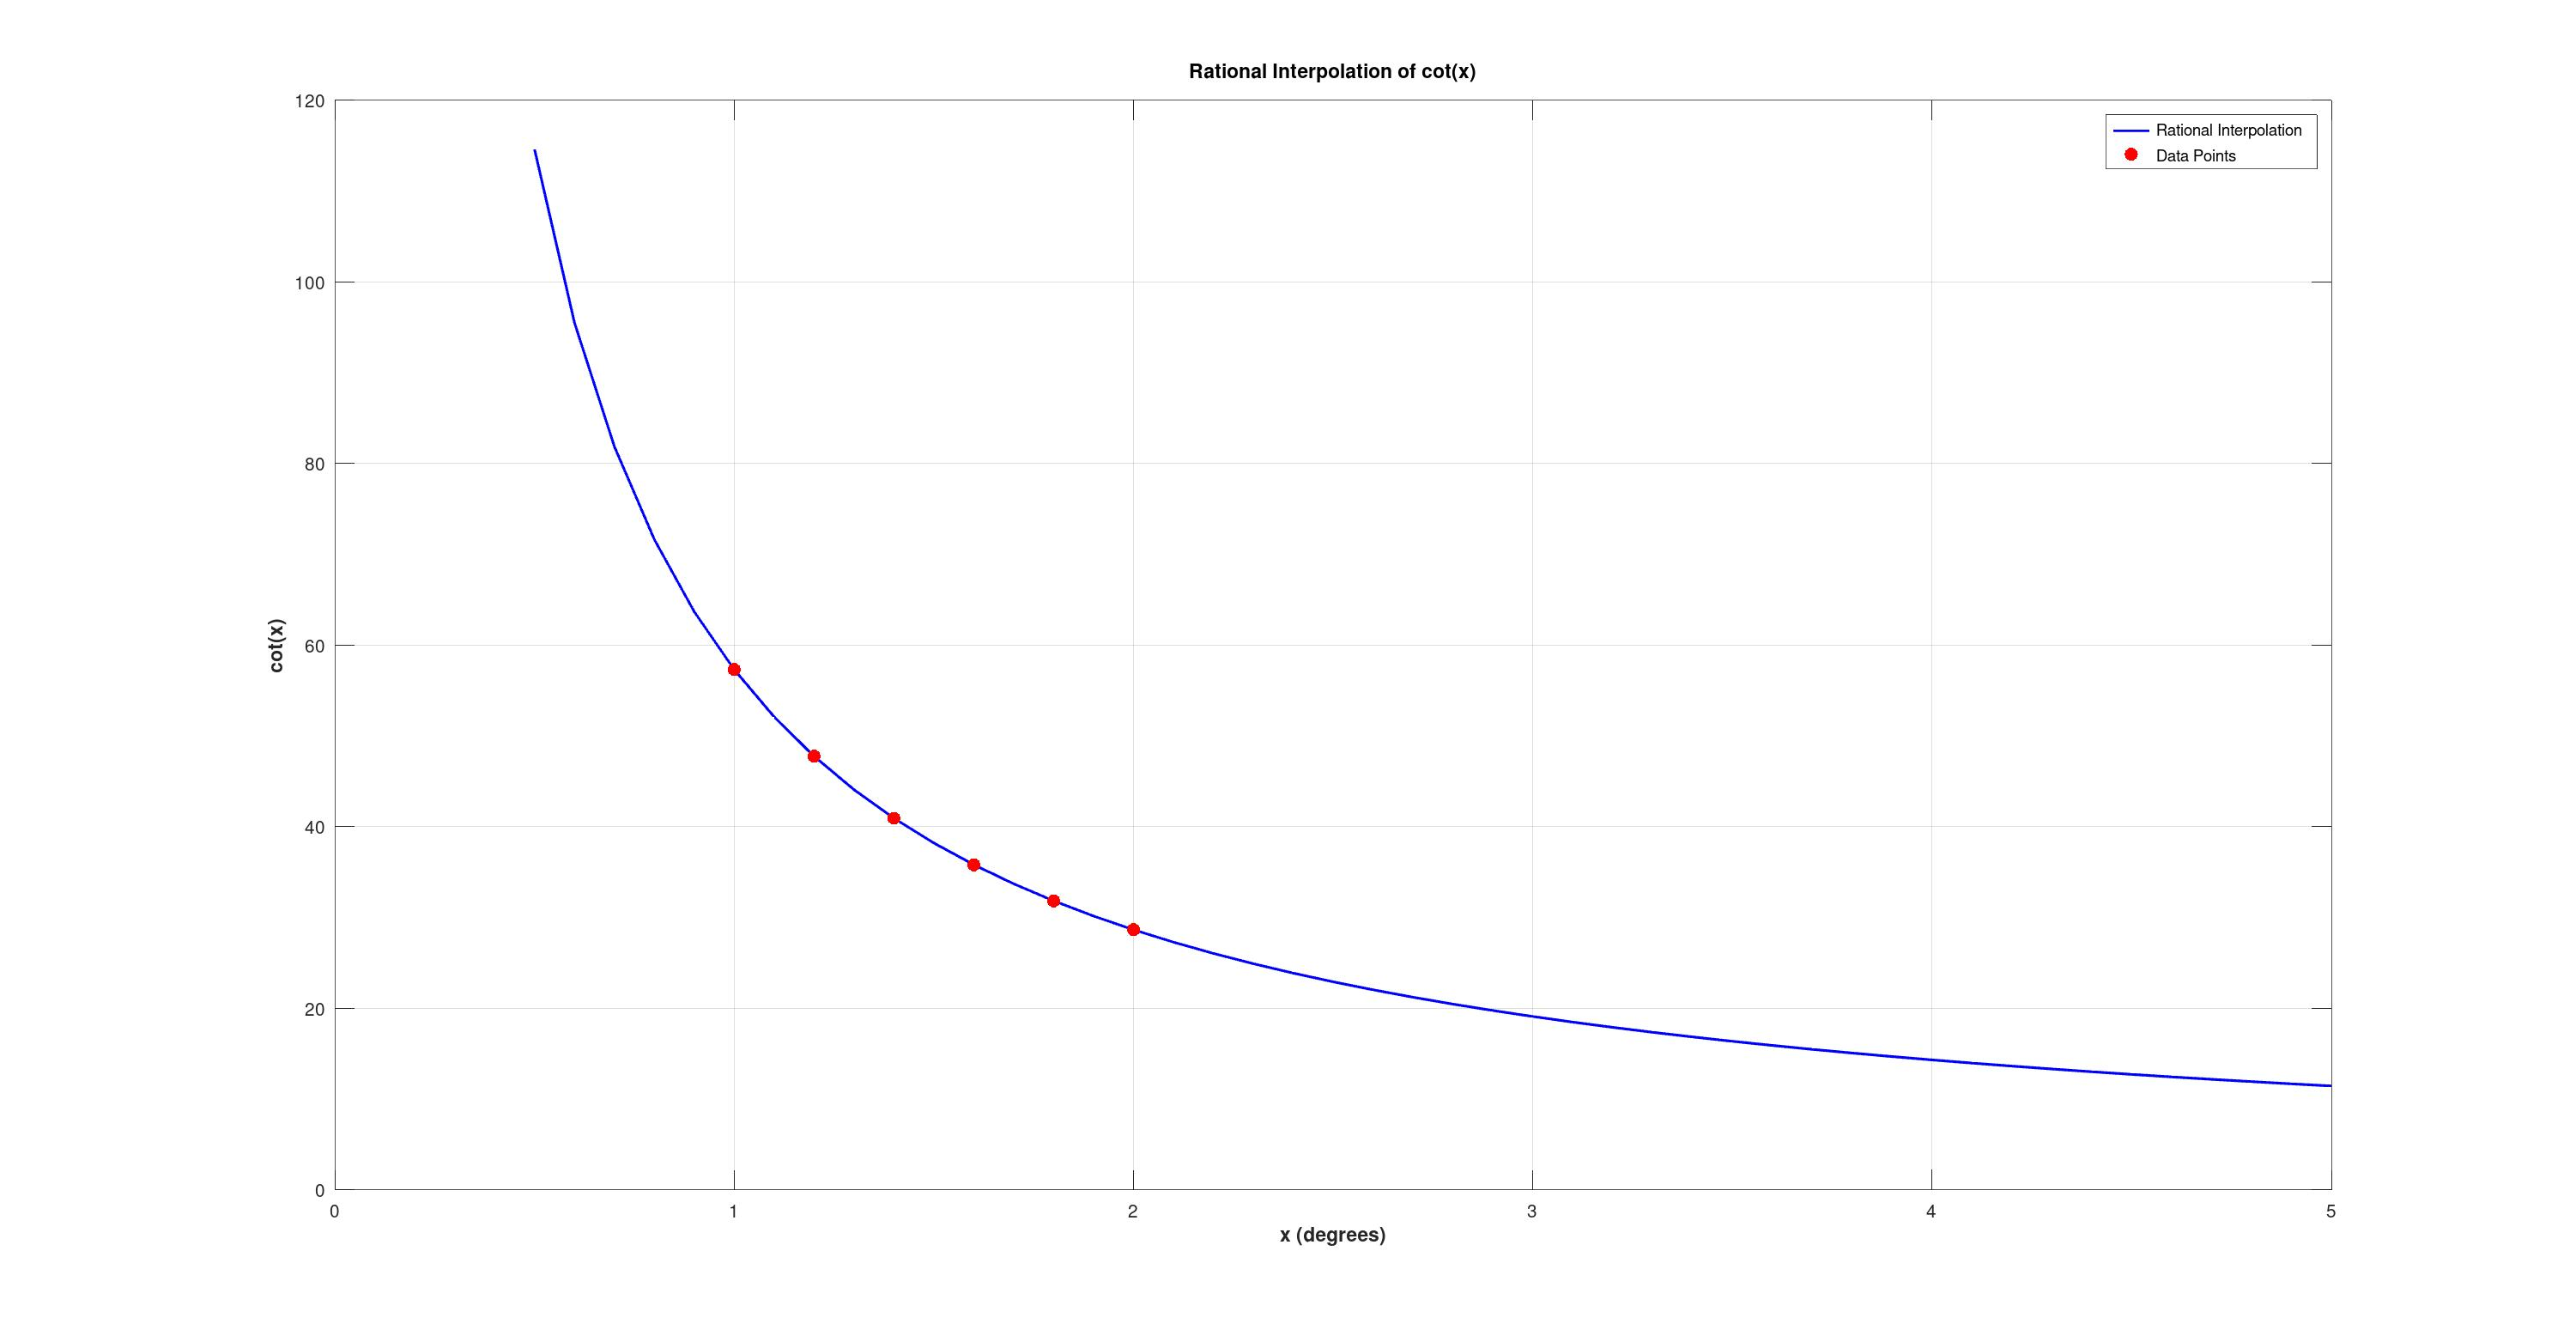
\includegraphics[width=0.93\textwidth]{a1.jpg}
  \caption{Rational interpolation of \(\cot(x)\) (blue line) and original sampled points (red circles).}
\end{figure}

\section*{Conclusion}
Rational interpolation successfully reconstructs the cotangent function from discrete samples, providing an accurate approximation even near singularities. The results at \(x=0.75^\circ\) show minimal deviation from the actual value. This demonstrates that rational interpolation is a reliable tool for approximating functions with rapidly varying or singular behavior.
